We work with directed, edge-labeled graphs admitting parallel edges. This notion differs from that of Barr and Wells \cite{barr1990category}, whose directed multigraphs with loops lack edge labels; from that of König et al. \cite{konig2018atutorial}, since we permit the collections of nodes and edges to be classes; and from that of Ehrig et al. \cite{ehrig1997handbook1}, where both nodes and edges are labeled, whereas here only edges are labeled.

Other notions of graphs appear in the literature for distinct purposes, including hypergraphs \cite{plump1993hypergraph}, attributed graphs \cite{ehrig2006fundamentals}, and polygraphs \cite{ara2023polygraphs}. Our choice reflects that a category in the sense of category theory (discussed in the next section) can be seen, in the style of Barr and Wells \cite{barr1990category}, as a directed edge-labeled multigraph endowed with extra structure, with object and morphism collections allowed to be classes.

\begin{definition}
    \label{def:graph}
     Let \(\Sigma\) be a finite set of labels. A \textbf{directed edge-labeled multigraph} is a structure \((V, E, \opn{dom}, \opn{cod},\lambda)\) where
    \begin{itemize}
        \item $V$ is a collection of distinct elements called \textbf{nodes} (or \textbf{objects}),
        \item $E$ is a collection of distinct elements, disjoint from $V$, called \textbf{edges} (or \textbf{arrows}),
        \item $\opn{dom}: E \mathop{\to} V$ is the \textbf{domain} (or \textbf{source}) function assigning to each edge its source node,
        \item $\opn{cod}: E \mathop{\to} V$ is the \textbf{codomain} (or \textbf{target}) function assigning to each edge its target node,
        \item $\lambda: E \mathop{\to} \Sigma$ is the \textbf{labeling} function assigning to each edge a label from $\Sigma$.
    \end{itemize}
    A directed edge-labeled multigraph is said to be \textbf{finite} if $V$ and $E$ are finite, and \textbf{discrete} if its edge set \(E\) is empty.
    For a directed edge-labeled multigraph \( G \), we write \( V(G) \) for its set of nodes, \( E(G) \) for its set of edges, \( \opn{dom}_G \) for its domain function, \( \opn{cod}_G \) for its codomain function, and \( \lambda_G \) for its labeling function. $a : s\overset{l}{\rightarrow} t$ denotes an arrow $a$ labeled by $l$ from $s$ to $t$.
\end{definition}
A directed edge-labeled multigraph may have multiple edges from one node to another, as well as loops (edges from a node to itself), because different edges $u,v$ can have the same source and target nodes, i.e. $\opn{dom}(u) \mathop{=} \opn{dom}(v)$ and $\opn{cod}(u) \mathop{=} \opn{cod}(v)$.

    Throughout, a directed edge-labeled multigraph will be simply referred to as a \enquote{labeled graph} or \enquote{graph} when the context makes it clear, and we fix a set $\Sigma$ of labels.

% \begin{definition} 
%     \label{def:graph}
%     Let \(\Sigma\) be a finite set of labels. A \textbf{directed edge-labeled multigraph} is an ordered pair \((G,\lambda)\) where \( G \) is an unlabeled graph and \( \lambda : E(G) \mathop{\rightarrow} \Sigma\) is an edge-labeling function. 
%     It is called \textbf{finite} if its underlying unlabeled graph is finite.
%     Throughout, a directed edge-labeled multigraph will be simply referred to as a \enquote{labeled graph} when the context makes it clear.
%     An arrow $a$ labeled by $l$ from $s$ to $t$ is denoted by $a : s\overset{l}{\rightarrow} t$.
% \end{definition}
%  The definition of labeled graphs extends the definition of unlabeled graphs, as unlabeled graphs can be seen as labeled graphs with a single label for all edges, i.e., the label function is a constant function.


\begin{example}
    Consider the graph shown 
    below.
    % in Figure~\ref{fig:preliminaries:labeled_graph}.
    It has two nodes which are marked with numbers to facilitate discussion, but in general, nodes are not labeled.
    There are five edges: two loops on node $1$ labeled \(a\) and \(b\), two edges from node $1$ to node $2$ both labeled \(a\), and one edge from node $2$ to node $1$ labeled \(a\). Note that the two edges from node $1$ to node $2$ are distinct edges, even though they share the same source, target, and label.

    % \begin{figure}[H]
    %    \centering
    \begin{center}
       \resizebox{0.4\textwidth}{!}{
        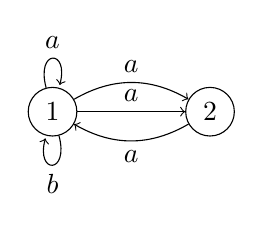
\begin{tikzpicture}
            \graphbox{}{0mm}{0mm}{32mm}{28mm}{-10mm}{-14mm}{
                \node[draw,circle] (1) at (0,0) {1};
                \node[draw,circle] (2) at (2,0) {2};
                \draw[->] (1) edge[loop above] node[midway, above] {$a$} (1) ;
                \draw[->] (1) edge[loop below] node[midway, below] {$b$} (1) ;
                \draw[->] (1) edge[bend left] node[midway, above] {$a$}  (2)  ;
                \draw[->] (1) edge node[midway, above] {$a$}  (2)  ;
                \draw[->] (2) edge[bend left] node[midway, below] {$a$} (1)   ;
            }
        \end{tikzpicture}
       }
    %     \caption{Labeled graph.}
    %     \label{fig:preliminaries:labeled_graph}
    % \end{figure}
    \end{center}


\end{example}
  A homomorphism of labeled graphs is a homomorphism of unlabeled graphs that preserves the labels assigned to the edges. 